\documentclass{article}

\usepackage[margin=2cm]{geometry}
\usepackage{makecell}
\usepackage{graphicx}
\usepackage{float}
\usepackage{caption}

\begin{document}
\hbox{
	\hspace*{0.08\textwidth}
	\rule{0.5pt}{\textheight}
	\hspace*{0.001\textwidth}
	\rule{0.5pt}{\textheight}
	\hspace*{0.05\textwidth}
	\parbox[b]{0.75\textwidth}{
		{\noindent\huge\bfseries Problem Analysis \& Software Design \\}\\[2\baselineskip] % Title
		\large{
		\textbf{Group:} 9\\[\baselineskip]
		\begin{tabular}{@{}l l l l@{}}
			\textbf{Names:}& Robbin de Groot  &\textbf{S-number:} &s3376508\\
			& Oliver Strik  & &s3100693\\
			& Nicu Ghidirimischi & &
		\end{tabular}}\\

		\vspace{6pt}
		{\large \textbf{Report:} Iteration 1 } \\[\baselineskip] % Tagline or further description
		{\large \textbf{Date:} \today } \\[4\baselineskip] % Tagline or further description
		{\large \textsc{ Prof. E.O. de Brock \& Dr. R. Smedinga }}
	\vspace{0.40\textheight} % Whitespace between the title block and the publisher
	{\Large\noindent \\ Computing Science - Year 2 \vspace{0.7cm}
	\Large\noindent \\University of Groningen \vspace{5pt}\\ \large Faculty of Science \& Engineering }}
}
\newpage

\vspace{1cm}
-- marked for change --
\section*{Introduction}
An auctioning company called ``The AuctionHouse\textsuperscript{TM}'' auctions provided goods to buyers. Currently, they auction and display the goods in a warehouse just outside of city limits. Owner John wants to automate the administration of auctions and other activities using an IT solution.

\vspace{1cm}
-- marked for change --
\section*{Expectations Summary and Conclusion}
John wants the sellers to be able to register their goods in the to-develop-system. These goods then need to be assessed and possibly removed if they lack the requirements. A couple of days before an auction, potential buyers must be able to view the goods. The goods are then auctioned at location (so not through the system).\\
Currently, regular customers get mail informing them of the goods on sale, rather than having to go and see the availlable goods in person.\\
Payments are done through cash or card, and not through credit cards. Bigger customers get offered a special billing procedure.
The police is handed a list of goods on auctions, so they can identify any stolen goods.
Once the system is completed, a system administrator should make sure every person has the right permissions for the system, and verify that it is operating properly.

\section*{Potential users and user wishes}
\subsection*{Actors and Users}
What follows is a list of user (groups) that need to interact with the system directly. The selection is derived from the above provided summary.
\begin{itemize}
	\item Owner of The AuctionHouse\textsuperscript{TM} (John)
	\item Private Individuals and Merchants (Owners of the goods)
	\item Purchasing agent
	\item Viewers
	\item System Administrator
\end{itemize}

\subsection*{Other Stakeholders}
Below is the list of people who have interests in the development of the system, or are otherwise involved with it, while not having to interface with it directly.
\begin{itemize}
	\item Regular Customer
	\item Big Customer
	\item Police
\end{itemize}

\subsection*{User Wishes and Stories}
Users and stakeholders need the system to be able to handle their requests. Below is a list of those wishes.
\begin{itemize}
	\item Administrators: do everything below under test environments
	\item Owner: add/remove/modify/view staff members
	\item Purchasing Agent: register/modify items for sale
	\item Auctioneer: mark item as sold
	\item Secretary: Add registers buyers and sellers to the system
	\item Secretary: Generate printouts of items for sale/sold/etc.
	\item Seller: view items they have for sale
	\item Seller: view items they have sold
	\item Buyer: view items they have bought
	\item Public: view items that are for sale
	\item Public: view auction schedule
\end{itemize}
To visualize this, we made a diagram. This diagram is a ``power tree'' that shows how permissions are divided and who can do the same as another user group.
\begin{figure}[H]
	\centering
	% ignore the compilation warning, it has to do with the pdf and the graphicx package not accounting for some variable within the file, even though the variable has had no purpose for about 10 years now. #research
	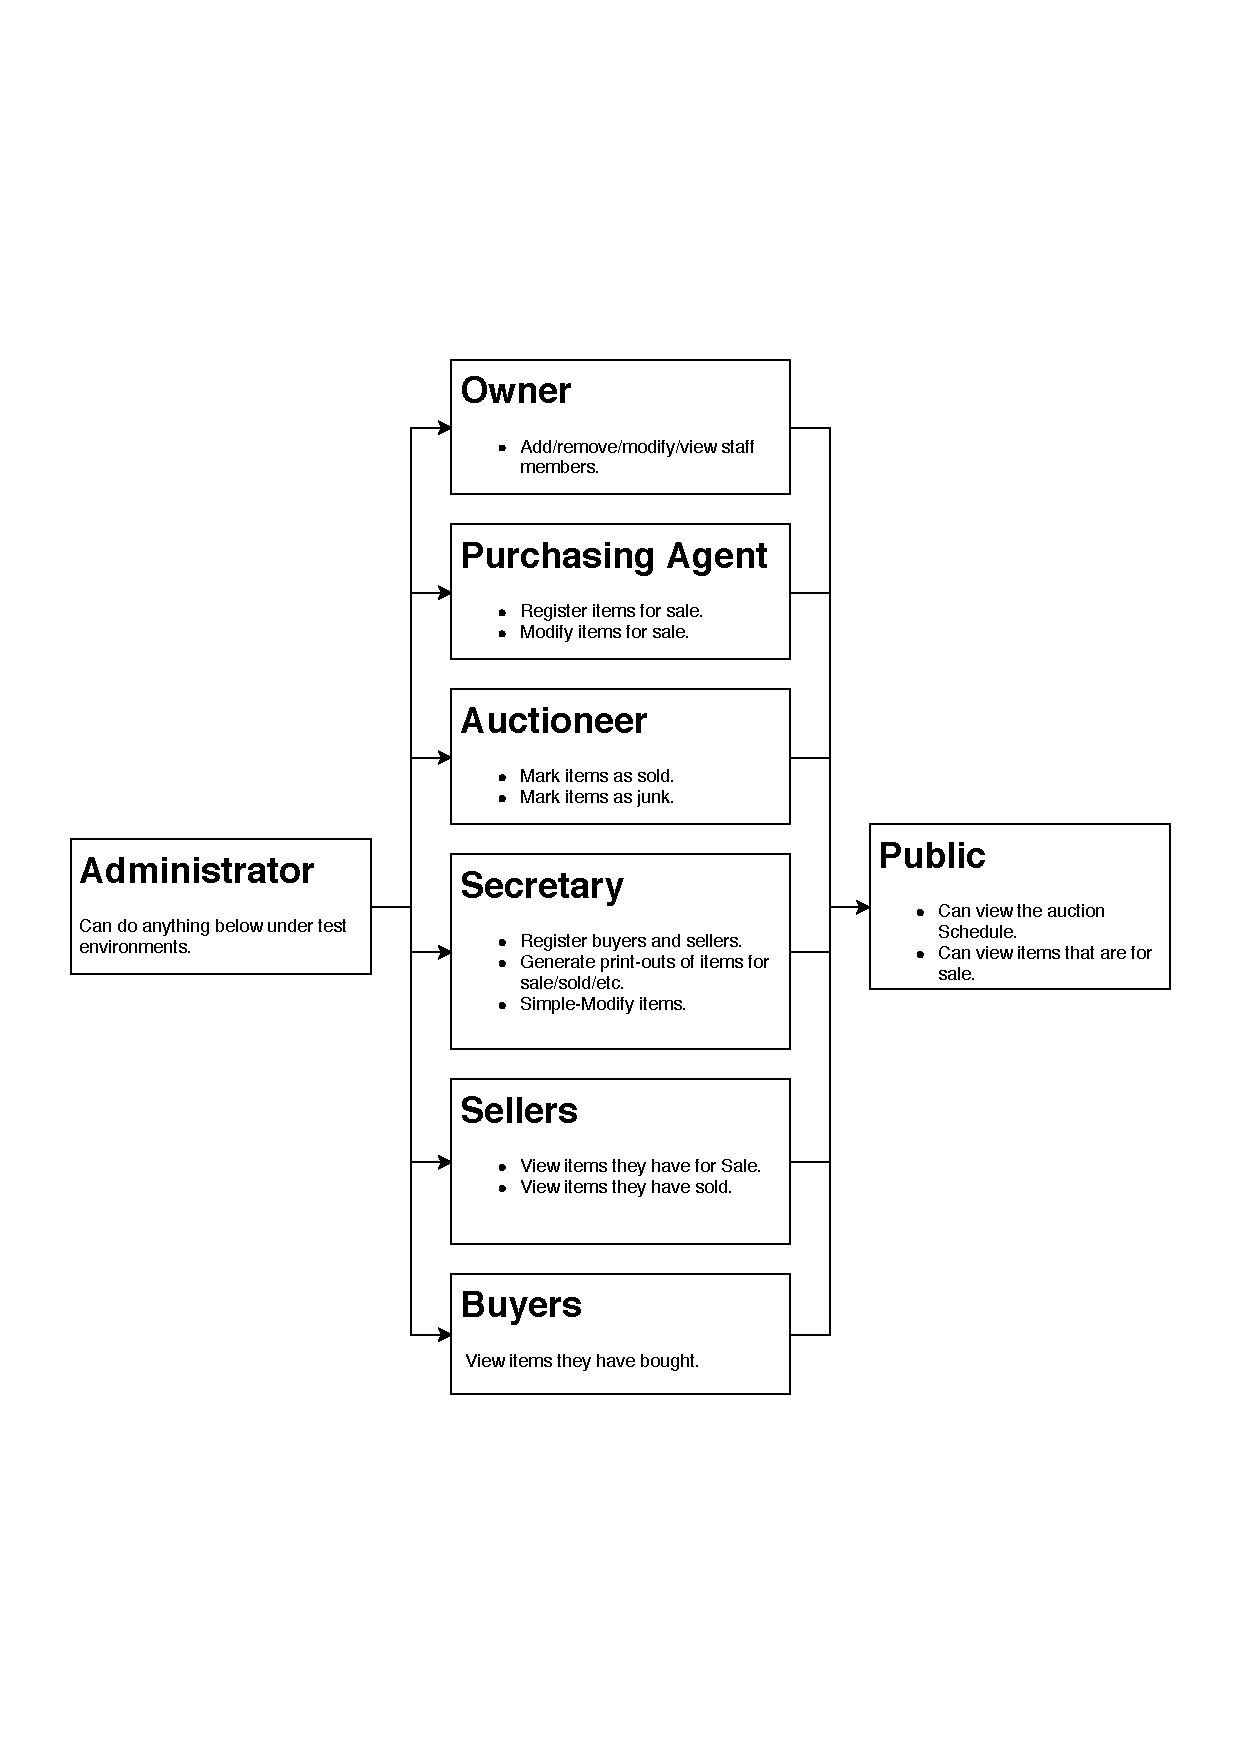
\includegraphics[scale=.75]{power_tree.pdf}
	\caption*{A power tree showing the relations between user groups and permissions. Arrows indicate what permissions are inherited}
\end{figure}

% Im not quite sure what is asked from us here. I emailed the helpdesk and let you know when I know more.
\section*{Use Cases}
\subsection*{Creating - Robbin de Groot}
\subsubsection*{Analysis}
\subsubsection*{Design}
\subsection*{Updating - Oliver Strik}
\subsubsection*{Analysis}
\subsubsection*{Design}
\subsection*{Deleting - Nicu Ghidirimischi}
\subsubsection*{Analysis}
\subsubsection*{Design}
\section*{Overall}
\section*{References}
\section*{About Possible Implementation (optional)}

% \begin{tabular}{l|l|c}
% User & Wish & CRUD\\\hline\hline
% \makecell[l]{Private Individuals\\Merchants} & Register Goods & \textbf{C}RUD
% Purchasing Agent & Assess goods for sale & C\textbf{R}U\textbf{D}

% \end{tabular}
\end{document}